\documentclass[a4paper]{article}
\usepackage[affil-it]{authblk}
\usepackage[english]{babel}
\usepackage[backend=bibtex,style=numeric]{biblatex}

\usepackage{geometry}
\geometry{margin=1.5cm, vmargin={0pt,1cm}}
\setlength{\topmargin}{-1cm}
\setlength{\paperheight}{29.7cm}
\setlength{\textheight}{25.3cm}

% useful packages.
\usepackage{amsfonts}
\usepackage{amsmath}
\usepackage{amssymb}
\usepackage{amsthm}     
\usepackage{enumerate} %enumerate environment
\usepackage{graphicx}
\usepackage{multicol}
\usepackage{fancyhdr}
\usepackage{layout}
\usepackage{ctex}      %中文环境
\usepackage{booktabs}  %三线表
\usepackage{verbatim}  %comment environment
\usepackage{float}     %强制表格图片位置
\usepackage{listings}  %insert code in latex
\usepackage{fontspec}  %font support
\usepackage{tikz}
\usepackage{makecell}
\usetikzlibrary{intersections}
\usepackage{arydshln}
\usepackage{mathptmx}
\usepackage{helvet}
\usepackage{courier}
\usepackage[colorlinks,linkcolor=blue]{hyperref}
\usepackage{xcolor}
\definecolor{mygreen}{rgb}{0,0.6,0}
\definecolor{lightgrey}{rgb}{0.95,0.95,0.95}
\definecolor{winered}{rgb}{0.5,0,0}
\definecolor{mymauve}{rgb}{0.58,0,0.82}
\lstset{
      backgroundcolor=\color{lightgrey},
      basicstyle             = \ttfamily,
      breakatwhitespace      = false,
      breaklines             = true,
      captionpos             = none,
      commentstyle           = \color{mygreen}\bfseries,
      extendedchars          = false,
      keepspaces             = true,
      keywordstyle           = \color{winered},         % keyword style
      language               = Python,                     % the language of code
      otherkeywords          = {string},
      numberstyle            = \tiny\color{mygray},
      rulecolor              = \color{black},
      showspaces             = false,
      showstringspaces       = false,
      showtabs               = false,
      stepnumber             = 1,
      stringstyle            = \color{mymauve},         % string literal style
      tabsize                = 2,
      title                  = \lstname,
      aboveskip              = 0pt,
      belowskip              = 0pt,
      columns                = flexible
}

% some common command
\newcommand{\dif}{\mathrm{d}}
\newcommand{\avg}[1]{\left\langle #1 \right\rangle}
\newcommand{\norm}[1]{\left\| #1 \right\|}
\newcommand{\difFrac}[2]{\frac{\dif #1}{\dif #2}}
\newcommand{\pdfFrac}[2]{\frac{\partial #1}{\partial #2}}
\newcommand{\OFL}{\mathrm{OFL}}
\newcommand{\UFL}{\mathrm{UFL}}
\newcommand{\fl}{\mathrm{fl}}
\newcommand{\op}{\odot}
\newcommand{\Eabs}{E_{\mathrm{abs}}}
\newcommand{\Erel}{E_{\mathrm{rel}}}
\addbibresource{citation.bib}

\begin{document}
% =================================================
\title{作业1报告}

\author{钱周越 3220104074
  \thanks{Electronic address: \texttt{3220104074@edu.zju.cn}}}
  
\affil{(Information and Computational Science Class 2201), Zhejiang University }


\date{Due time: \today}

\maketitle

\section{问题描述}
本报告旨在对四个股票因子——`return\_1m`、`turn\_1m`、`std\_1m` 和 `std\_FF3factor\_1m`——进行分析，以评估其预测股票收益的能力。具体任务包括：
\begin{itemize}
    \item 构建股票池：每月末剔除上市不满 252 个交易日的股票、已退市股票以及停牌股票。
    \item 计算因子值：对筛选后的股票池计算四个因子的原始值。
    \item 因子预处理：对因子值进行去极值、行业市值中性化和标准化处理。
    \item 因子测试：通过 RankIC 法和分层测试法评估因子的预测效果。
    \item 结果呈现：输出因子值、RankIC 时间序列、分层收益率序列，并绘制累计 RankIC 和分层收益率图。
\end{itemize}

\section{方法}

\subsection{股票池筛选}
\begin{itemize}
    \item \textbf{剔除标准}：剔除上市不满 252 个交易日的股票、已退市股票以及月末截面日停牌的股票（停牌判断标准为当日成交额为 0）。
    \item \textbf{月度横截面}：每月末更新股票池并进行因子计算。
\end{itemize}

\subsection{因子计算}
\begin{itemize}
    \item \textbf{return\_1m}：最近 21 个交易日的累计收益率。
    \item \textbf{turn\_1m}：最近 21 个交易日内每日换手率的均值。
    \item \textbf{std\_1m}：最近 21 个交易日内每日收益率的标准差。
    \item \textbf{std\_FF3factor\_1m}：最近 21 个交易日内，日收益率序列对中证全指日收益率、SMB 因子日收益率、HML 因子日收益率序列进行多元线性回归的残差的标准差。
\end{itemize}

\subsection{因子预处理}
\begin{itemize}
    \item \textbf{去极值}：将因子值大于 \( \text{mean} + 3 \times \text{std} \) 的值设为 \( \text{mean} + 3 \times \text{std} \)，小于 \( \text{mean} - 3 \times \text{std} \) 的值设为 \( \text{mean} - 3 \times \text{std} \)。
    \item \textbf{行业市值中性化}：以去极值后的因子值为因变量，以 A 股市值因子（流通市值取对数、去极值、zscore 标准化）和中信一级行业哑变量为自变量，进行 OLS 多元线性回归，取残差。
    \item \textbf{标准化}：对因子值进行 zscore 标准化，使其均值为 0，标准差为 1。
\end{itemize}

\subsection{因子测试}
\begin{itemize}
    \item \textbf{RankIC}：计算因子值与下个月收益率的 Spearman 相关系数。
    \item \textbf{分层测试}：将因子值降序排列，分为 5 层（每层 20\%），计算每层股票下个月的等权收益率。
\end{itemize}

\section{结果}

\subsection{因子值}
\begin{itemize}
    \item \textbf{原始因子值与预处理后的因子值}：分别存储在 `factors\_raw.csv` 和 `factors\_processed.csv` 文件夹中。以因子名命名。
\end{itemize}

\subsection{RankIC 与分层收益率}
\begin{itemize}
    \item \textbf{RankIC 时间序列}和\textbf{分层收益率时间序列}：存储在'factor\_test\_results'文件夹中。以因子名命名。
\end{itemize}

\subsection{累计 RankIC 与分层收益率}
下面是所画的分层收益图和累计 RankIC 图。
\begin{enumerate}
    \item \textbf{return\_1m}：\par
    \begin{figure}[H]
        \centering
        \begin{minipage}{0.45\textwidth}
            \centering
            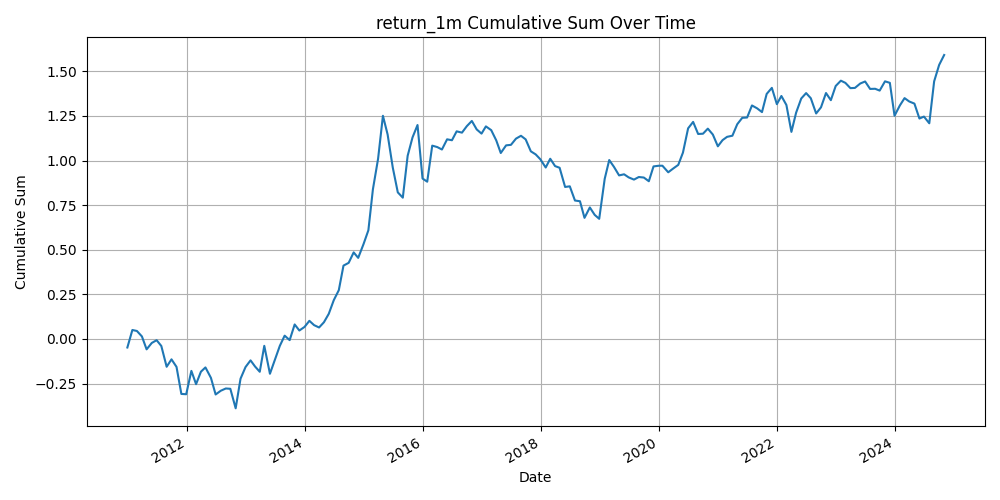
\includegraphics[width=\textwidth]{../over time plot/return_1m_cumsum.png}
            \caption{分层系数}
        \end{minipage}\hfill
        \begin{minipage}{0.45\textwidth}
            \centering
            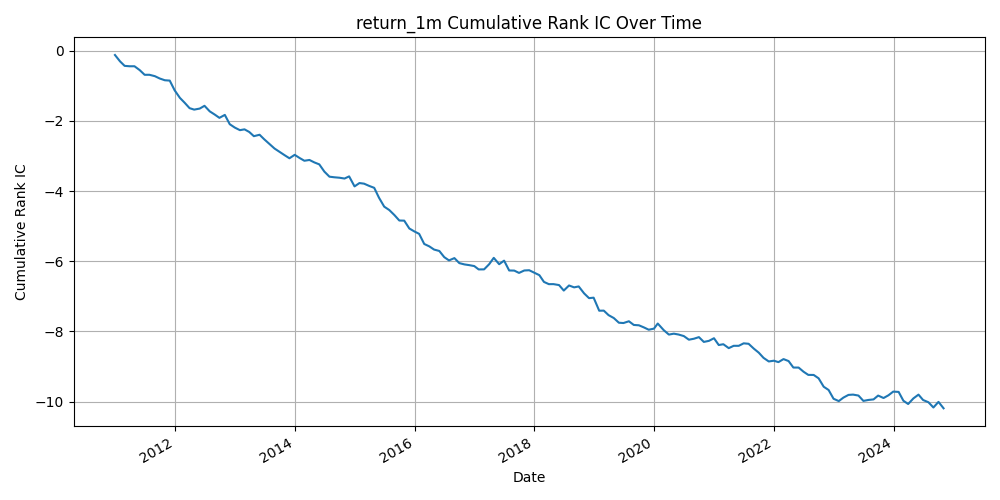
\includegraphics[width=\textwidth]{../over time plot/return_1m_rank_ic_cumsum.png}
            \caption{RankIC}
        \end{minipage}
      \end{figure}
    \item \textbf{turn\_1m}：\par
    \begin{figure}[H]
        \centering
        \begin{minipage}{0.45\textwidth}
            \centering
            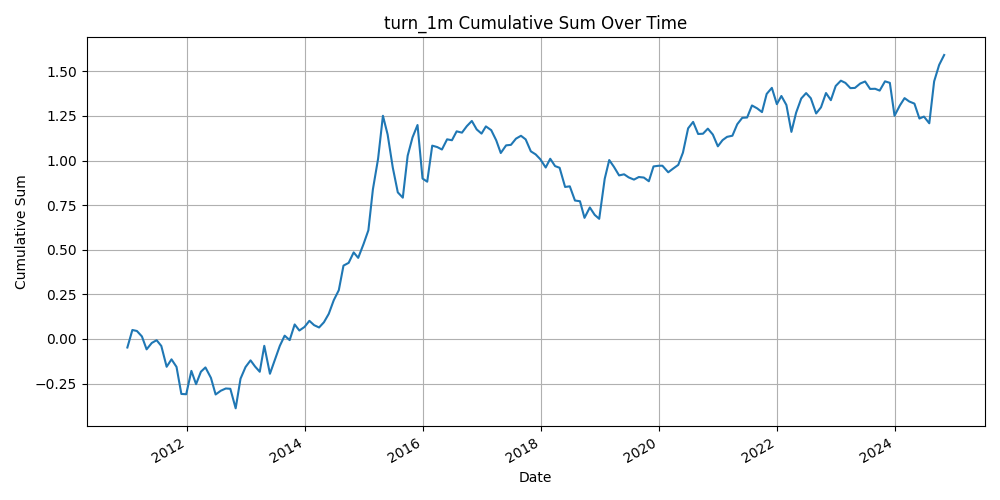
\includegraphics[width=\textwidth]{../over time plot/turn_1m_cumsum.png}
            \caption{分层系数}
        \end{minipage}\hfill
        \begin{minipage}{0.45\textwidth}
            \centering
            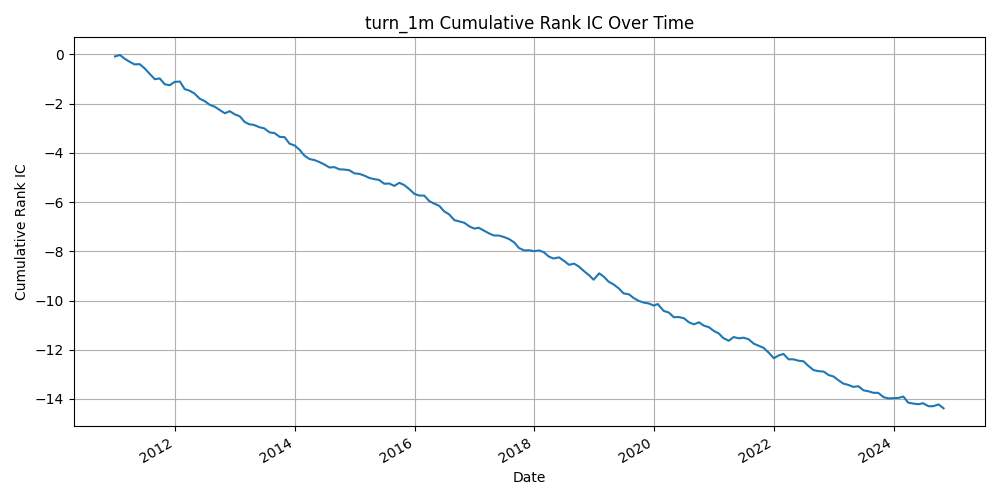
\includegraphics[width=\textwidth]{../over time plot/turn_1m_rank_ic_cumsum.png}
            \caption{RankIC}
        \end{minipage}
      \end{figure}
    \item \textbf{std\_1m}：\par
    \begin{figure}[H]
        \centering
        \begin{minipage}{0.45\textwidth}
            \centering
            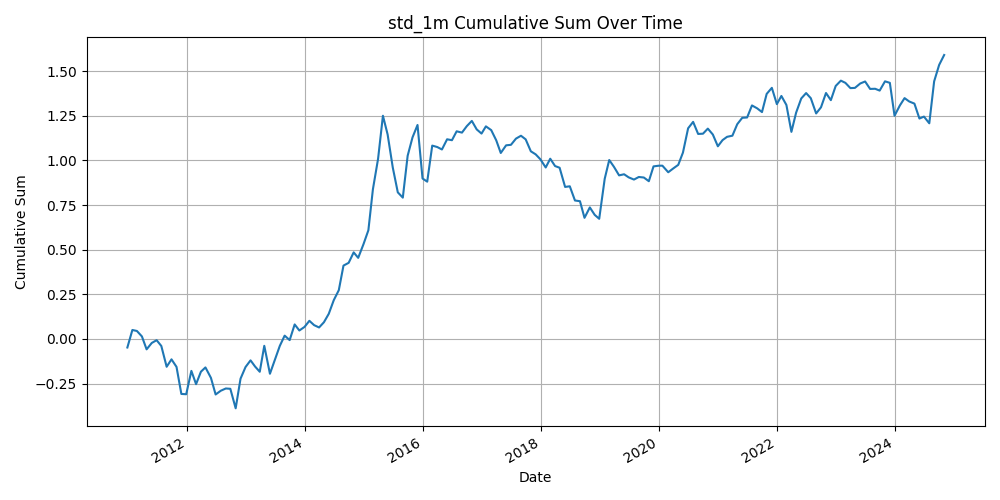
\includegraphics[width=\textwidth]{../over time plot/std_1m_cumsum.png}
            \caption{分层系数}
        \end{minipage}\hfill
        \begin{minipage}{0.45\textwidth}
            \centering
            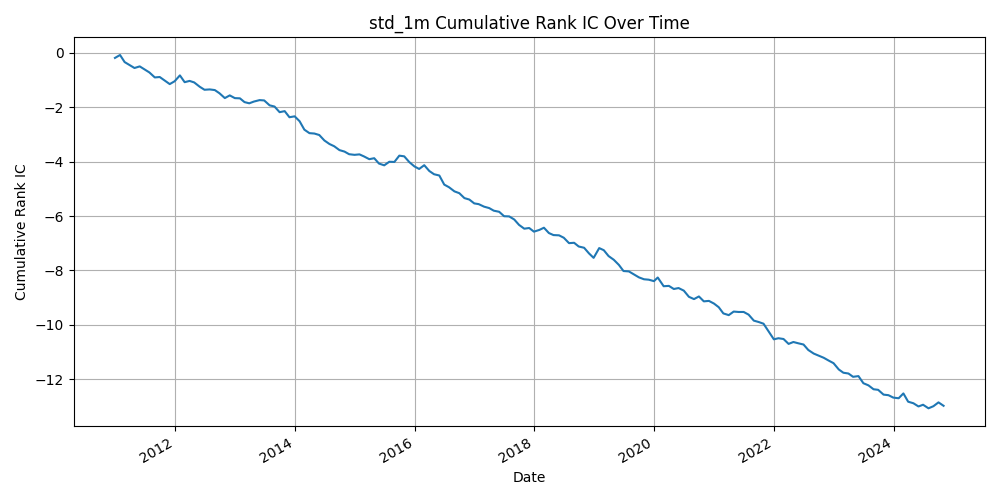
\includegraphics[width=\textwidth]{../over time plot/std_1m_rank_ic_cumsum.png}
            \caption{RankIC}
        \end{minipage}
      \end{figure}
    \item \textbf{std\_FF3factor\_1m}：\par
    \begin{figure}[H]
        \centering
        \begin{minipage}{0.45\textwidth}
            \centering
            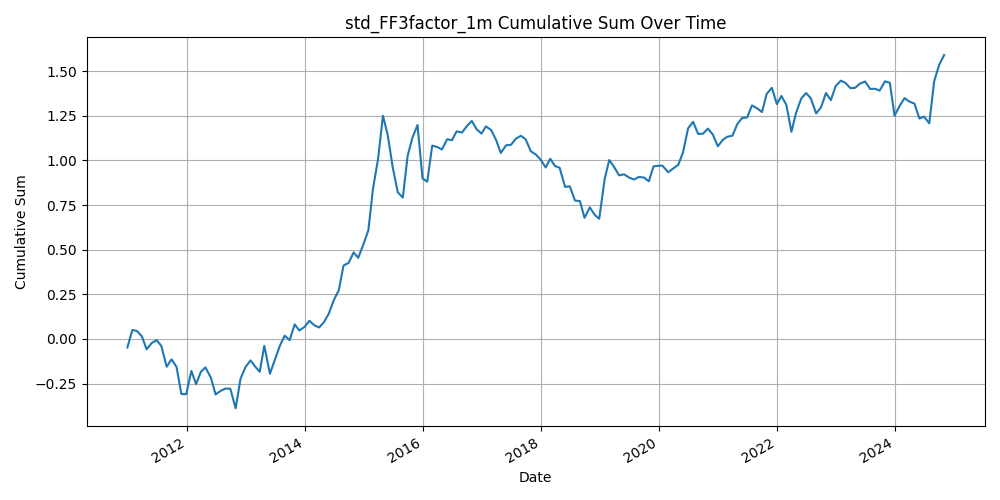
\includegraphics[width=\textwidth]{../over time plot/std_FF3factor_1m_cumsum.png}
            \caption{分层系数}
        \end{minipage}\hfill
        \begin{minipage}{0.45\textwidth}
            \centering
            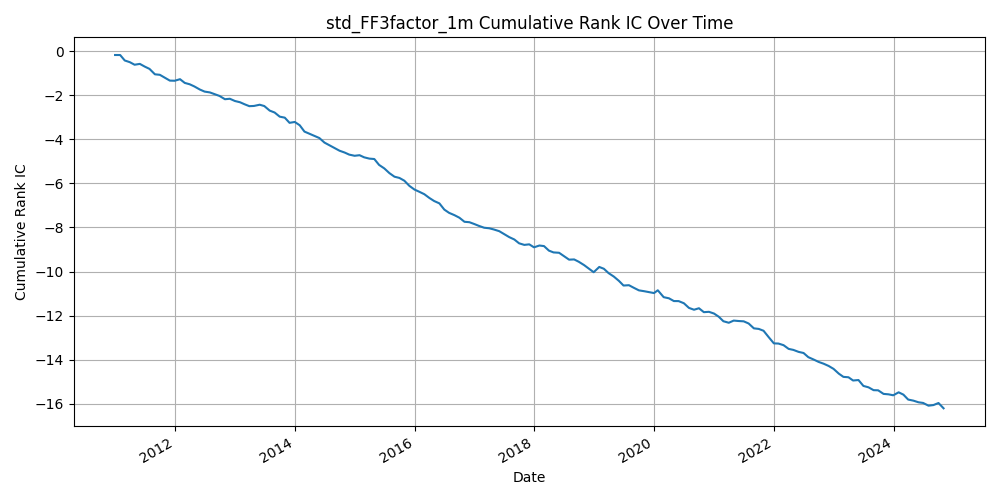
\includegraphics[width=\textwidth]{../over time plot/std_FF3factor_1m_rank_ic_cumsum.png}
            \caption{RankIC}
        \end{minipage}
      \end{figure}
\end{enumerate}





\end{document}